\chapter{Parking Lot}
\label{ch:lot}

\section{Accelerator / Sytem Integration}

The degree to which these accelerators are integrated with the host system varies.
Figure~\ref{fig:integration-spectrum} depicts how integrated some common accelerators are.
Fully-integrated accelerators are characterized by direct and transparent access to system memory, no additional programming system or compiler support, and no explicit control through an OS or vendor API.
For example, floating-point accelerators are fully integrated.
They have migrated into the host instruction-set architecture, have first-class access to system memory, and are supported without specialized toolchains or programming systems.
Similarly, SIMD vector extensions are nearly as integrated, but may require some special attention to memory alignment, precision, or rounding modes.
In contrast, fully-discrete accelerators have their own memory, have esoteric programming systems, and demand explicit control.
For example, FPGAs are programmed in hardware-description languages, may require the host system to be rebooted to be reconfigured, and often require the programmer to explicity transfer data to their memory.
As on the of the most mature accelerators, GPUs occupy a middle ground.
GPUs vary from partially-integrated to discrete: when a GPU is integrated on the same die as the CPU, it may share the same physical memory, but the computation model remains for compute tasks to be ``offloaded'' to the GPU, with the CPU managing the execution.

\begin{figure}
    \centering
    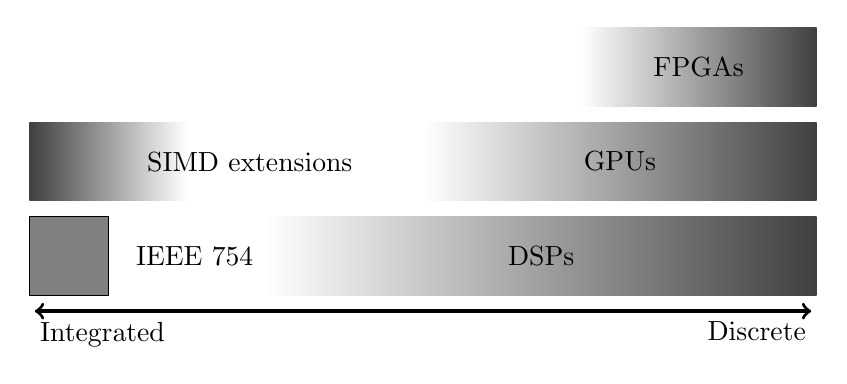
\begin{tikzpicture}[
        nodestyle/.style={},
        axisline/.style={
            <->,
            very thick,
            shorten <=2pt,
            shorten >=2pt,},
        axistext/.style={},
        ]

        \pgfmathsetmacro{\rt}{1} % thickness
        \pgfmathsetmacro{\rs}{0.2} % spacing

        \pgfmathsetmacro\ra{\rs}
        \pgfmathsetmacro\rb{\ra+\rt+\rs}
        \pgfmathsetmacro\rc{\rb+\rt+\rs}


        \draw[axisline] (0,0) node[anchor=north west] {Integrated} -- (10,0) node[anchor=north east] {Discrete};

        \draw[fill=gray] (0,\ra) rectangle (1,\ra+\rt);
        \node [above] at (2.1, \ra+0.25\rt) {IEEE 754};

        \shade[left color=darkgray, right color=white] (0,\rb) rectangle (2,\rb+\rt);
        \node [above] at (2.8, \rb+0.25\rt) {SIMD extensions};

        \shade[left color=white, right color=darkgray] (3,\ra) rectangle (10,\ra+\rt) node[pos=0.5] {DSPs};
        \shade[left color=white, right color=darkgray] (5,\rb) rectangle (10,\rb+\rt) node[pos=0.5] {GPUs};
        \shade[left color=white, right color=darkgray] (7,\rc) rectangle (10,\rc+\rt) node[pos=0.5] {FPGAs};

    \end{tikzpicture}
    \caption{Spectrum of integration for accelerators.}
    \label{fig:integration-spectrum}
\end{figure}